\section{AI Agents}
% Chapter 2 — Section 4 (LaTeX)
% This file provides Section 4 of Chapter 2: "Introduction, Historical Foundations, and Architectures for LLM Agents"
% Citation numbering begins at [25] as requested (manual labels used for bibliography entries).
\label{ch2:sec4}

The concept of an \emph{intelligent agent} has been central to artificial intelligence (AI) since the field's earliest formulations.  Historically, the agent abstraction was introduced to formalize computational systems that \emph{sense} an environment, \emph{decide} on actions, and \emph{act} in order to achieve objectives or to reduce error according to some criterion.  This sense--think--act loop draws on intellectual antecedents that span multiple disciplines.  Norbert Wiener's foundational exposition of cybernetics emphasized feedback, control, and communication in both biological and engineered systems and thereby provided a formal vocabulary for thinking about closed-loop behavior that adapts to an environment \cite{wiener48}.  Early symbolic AI adopted and developed agent taxonomies and architectures oriented around planning, search, and knowledge representation; these symbolic systems relied on explicit rule sets, logical inference, and handcrafted world models to produce action sequences in constrained domains.  Complementing symbolic approaches, the study of natural language interaction—epitomized by Joseph Weizenbaum's ELIZA—demonstrated both the promise and the pitfalls of programmatic conversational behavior: ELIZA's pattern-matching and re-assembly rules generated the \emph{appearance} of dialogic competence while exposing the gap between surface textual fluency and semantically grounded, environment-anchored agency \cite{weizenbaum66}.  The interplay of these strands—feedback control (cybernetics), symbolic planning (classical AI), and rudimentary conversational interfaces—set the stage for later statistical and neural methods that would substantially change the substrate on which agents are built.

During the late twentieth and early twenty-first centuries, statistical and machine learning approaches matured into practical tools for perception and decision making.  Reinforcement learning (RL) formalized agent learning as the optimization of a cumulative return within an environment modeled as a Markov Decision Process (MDP) or, more generally, a partially observed MDP (POMDP).  Canonical methods—temporal difference learning, Q-learning, and actor-critic algorithms—provided the algorithmic foundations for training agents interacting sequentially with environments (see, e.g., the canonical text by Sutton and Barto).  The introduction of deep neural function approximators into RL—most prominently demonstrated by Deep Q-Networks (DQN) that learned to map raw pixel observations to actions with human-level performance on Atari games—showed that end-to-end learning could produce effective task-oriented controllers from high-dimensional sensory inputs \cite{mnih15,sutton98}.  Nonetheless, RL and earlier agentic systems were often \emph{narrow}: they were designed and optimized for specific tasks or domains, required substantial task-specific engineering (reward shaping, environment simulators), and typically lacked the flexible natural-language interface that characterizes modern open-ended human–machine interaction.

The advent of large pretrained language models (LLMs) in the 2010s and early 2020s created a new capability frontier.  Transformer architectures, introduced by Vaswani \emph{et~al.}, provided scalable, attention-based sequence models that could be trained efficiently on massive corpora and that learned long-range contextual dependencies critical to linguistic competence \cite{vaswani17}.  The paradigm of self-supervised pretraining followed by task-specific adaptation (fine-tuning or prompting) demonstrated that very large autoregressive or encoder–decoder models internalize rich linguistic, factual, and procedural priors that can be exploited in zero- and few-shot regimes; GPT-3, for example, empirically illustrated how scaling model size and pretraining data substantially improves generalization and in-context learning ability \cite{brown20}.  Concurrently, retrieval-augmented methods provided mechanisms for coupling parametric model knowledge with non-parametric external memories (e.g., dense passage retrieval), enabling models to consult large knowledge stores at inference time to reduce factual errors and to extend effective context beyond the model's token window \cite{lewis20}.

Together, these advances suggested a radical reconceptualization of agent design: rather than constructing narrowly engineered controllers, one could position LLMs as \emph{agentic cores} (``brains'') that combine broad world knowledge, language understanding, and flexible reasoning with engineered periphery components (memory stores, tool APIs, execution middleware) to realize richer autonomous behavior.  Starting circa 2022–2023, the research literature began to formalize this perspective and to introduce concrete methodologies for turning LLMs into autonomous or semi-autonomous agents.  Two influential motifs emerged in this literature: (i) \emph{tool augmentation}—training or prompting LLMs to decide when and how to call deterministic or specialized tools (calculators, search engines, code execution sandboxes) to improve accuracy and grounding \cite{schick23}; and (ii) \emph{reasoning–acting interleaving}—techniques that permit the model to produce explicit reasoning traces interleaved with action tokens, thereby enabling verification, iterative planning, and error correction (e.g., the ReAct paradigm) \cite{yao22}.  These developments reframed the old sense–think–act cycle: the LLM often serves simultaneously as an interpreter of natural language, a planner of multi-step procedures, and a controller that issues executable instructions, while external modules supply grounding and verifiable computation.

The remainder of this section surveys canonical architectural patterns for LLM agents found in contemporary research, formalizes their decision processes, and discusses practical mediation mechanisms such as retrieval-augmented generation and schema-based tool invocation.

\subsection{Architectural Taxonomy for LLM Agents}
\label{sec:architectures}

Contemporary LLM agent architectures can be characterized along a design spectrum that ranges from \emph{single-model policy agents} to \emph{modular planner–executor systems} and to \emph{tool-augmented hybrid systems}.  Each design exhibits distinct trade-offs in interpretability, sample efficiency, computational cost, and suitability for long-horizon tasks.

\subsubsection{Single-Model Policy Agents (LLM as a Policy)}
\label{sec:single_model}

The most straightforward architecture treats a pretrained LLM as a stochastic policy $\pi_{\theta}$ that maps a textual \emph{context} $c_t$ to a distribution over tokens, which are then parsed into higher-level \emph{actions} executed in the environment.  Formally, at discrete time step $t$ the model yields
\[
\text{token}_{t+1} \sim p_{\theta}(\cdot \mid c_t),
\]
and a higher-level action $a_t$ is obtained by deterministically parsing the emitted token sequence (for example, decoding a JSON object into an API call).  One may therefore express the induced policy over environment actions as
\begin{equation}\label{eq:policy_via_text}
  \pi_{\theta}(a_t \mid s_t) \;=\; \sum_{x \in \mathcal{T}(a_t)} p_{\theta}(x \mid c_t),
\end{equation}
where $\mathcal{T}(a_t)$ denotes the set of token sequences that parse to action $a_t$, and $s_t$ denotes the environment state (possibly only partially observed and implicitly represented within $c_t$).  Objective-wise, training or adapting such a policy aims to maximize an expected return,
\[
J(\theta) \;=\; \mathbb{E}_{\pi_\theta,\mathcal{E}}\!\left[\sum_{t=0}^T r_t\right],
\]
with $r_t$ the environment reward and the expectation taken over environment dynamics and the policy's stochasticity.

In practice, single-model policies are commonly augmented with retrieval systems (retrieval-augmented generation, RAG) to extend effective context beyond the architecture's maximum token window: a retrieval module returns a set of relevant documents or knowledge snippets which are concatenated (or summarized) into the prompt given to the model, thereby reducing hallucination and improving factual accuracy \cite{lewis20}.  Tool use is implemented through a middleware layer that maps specific token patterns to API invocations; recent work shows that models can be trained to \emph{decide} both \emph{when} to call a tool and \emph{how} to incorporate the tool's output into subsequent token prediction.  The Toolformer methodology is an example of a self-supervised procedure in which candidate API call sites are discovered and judged by their impact on language modeling likelihood, producing models that learn to employ calculators, search, Q\&A endpoints, and other utilities selectively \cite{schick23}.

\paragraph{Practical considerations.} Single-model policies are attractive for their simplicity and for minimizing engineering overhead: a single LLM instance, given a carefully designed prompt and a retrieval front end, can accomplish a wide range of tasks.  However, this design places the entire burden of multi-step planning, long-term state management, and error correction on token-level generation.  Token budget constraints limit how much historical context can be considered directly, and complex, safety-sensitive tool invocations require conservative validation middleware to avoid executing malformed or adversarially crafted actions.

\subsubsection{Modular Planner–Executor Architectures}
\label{sec:planner_executor}

A more robust and interpretable design decouples high-level planning from low-level execution by creating a hierarchical pipeline.  In this pattern, an LLM may serve as the \emph{planner} that emits a structured plan $P=\text{Plan}(c_t)$ consisting of subgoals $\{g_1,\dots,g_k\}$; each subgoal is then dispatched to an \emph{executor} (which may be another LLM with a focused prompt or a deterministic tool) that performs the concrete actions.  Concretely, the operational loop alternates:

\begin{enumerate}
  \item \textbf{Planner:} produce $P_k = \text{LLM}_{\mathrm{plan}}(c_t)$, a plan expressed in natural language or in a structured schema (e.g., a sequence of API calls).
  \item \textbf{Executor:} for each subgoal $g \in P_k$, invoke an executor module (specialized LLM or deterministic function) to carry out $g$, obtaining outcome $o_g$.
  \item \textbf{Feedback:} aggregate $\{o_g\}$ into an updated context $c_{t+1}$ and replan if necessary.
\end{enumerate}

This decomposition affords several technical advantages.  First, it improves interpretability: intermediate plans and subgoal outcomes are explicit and inspectable, enabling human audits or automatic verification checks.  Second, it enables targeted fine-tuning: the planner and executor may be adapted independently (for example, use a smaller specialized model for deterministic execution tasks while retaining a larger model for high-level planning).  Third, hierarchical control facilitates retries and conditional branching: if an executor fails, the planner can revise the plan based on the observed failure mode.

A particularly effective variant interleaves explicit \emph{reasoning traces} with actions; this is the design principle behind the ReAct paradigm.  In ReAct, the LLM alternates between producing \emph{reasoning tokens} $r_t$ (chain-of-thought style traces that document internal deliberation) and \emph{action tokens} $a_t$ (which may correspond to tool calls or textual actions).  Symbolically one may write the trajectory as
\[
[r_1, a_1, r_2, a_2, \ldots] \sim \pi_\theta(\cdot \mid c_t),
\]
and empirical evidence suggests that producing explicit, human-interpretable reasoning traces while acting improves both performance and debuggability on tasks that require multi-step planning and interaction with external knowledge sources \cite{yao22}.

\paragraph{Training regimes.} Modular agents are typically trained using a mixture of supervised fine-tuning on (context, plan, execution) triples and reinforcement learning where planners are scored based on downstream executor outcomes.  The modularity reduces the scale of data required for each subcomponent and allows for curriculum design in which simpler plans are learned first and complexity gradually increases.


\begin{figure}[t]
  \centering
  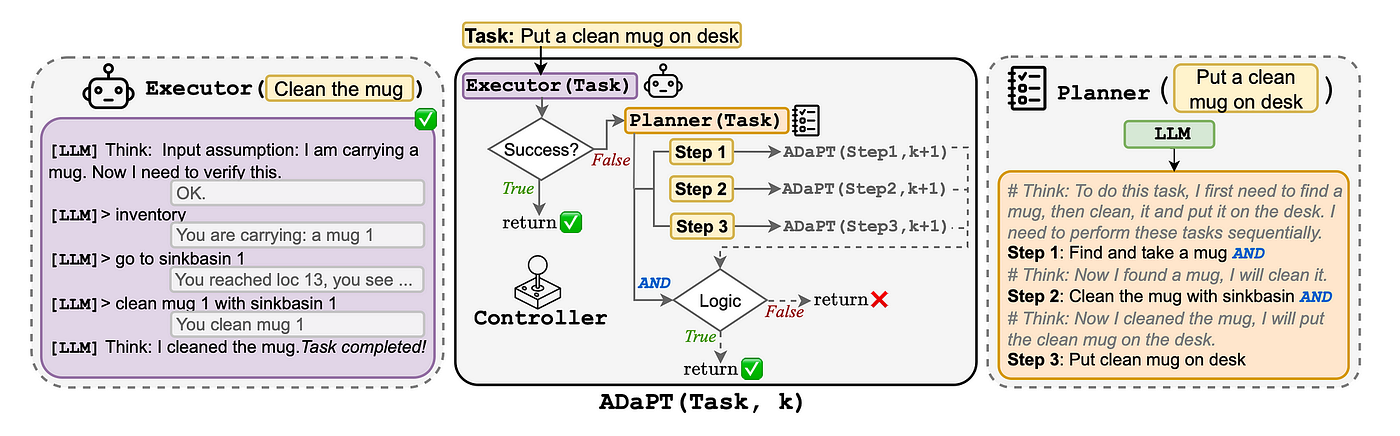
\includegraphics[width=0.85\linewidth]{images/ai/planner_executer_plus.png}
  \caption{Planner--Executor architecture for schema generation.}
  \label{fig:planner-executor}
\end{figure}


\subsubsection{Tool-Augmented and Meta-Learned Tool Use}
\label{sec:tools}

A dominant engineering pattern for high-fidelity agent behavior is explicit \emph{tool augmentation}.  In this design, a set $\mathcal{U}=\{u_1,\dots,u_m\}$ of external utilities (search, calculator, code runner, database queries, domain APIs) is registered with the agent platform.  The LLM learns (or is prompted) to select an element $u\in\mathcal{U}$ and to provide schema-conforming arguments; middleware then invokes $u$, and its output is reintegrated into the prompt or into a memory store.  The canonical pipeline is:

\begin{enumerate}
  \item \textbf{Parse:} map a structured subsequence of tokens to an API call $\mathrm{call}(u;\, \alpha)$ where $\alpha$ denotes arguments.
  \item \textbf{Invoke:} execute the tool in a sandboxed runtime, returning output $o_u$.
  \item \textbf{Embed:} convert $o_u$ to text and/or vector embeddings, and insert into the agent's context (possibly after summarization) for subsequent steps.
\end{enumerate}

\begin{figure}[t]
  \centering
  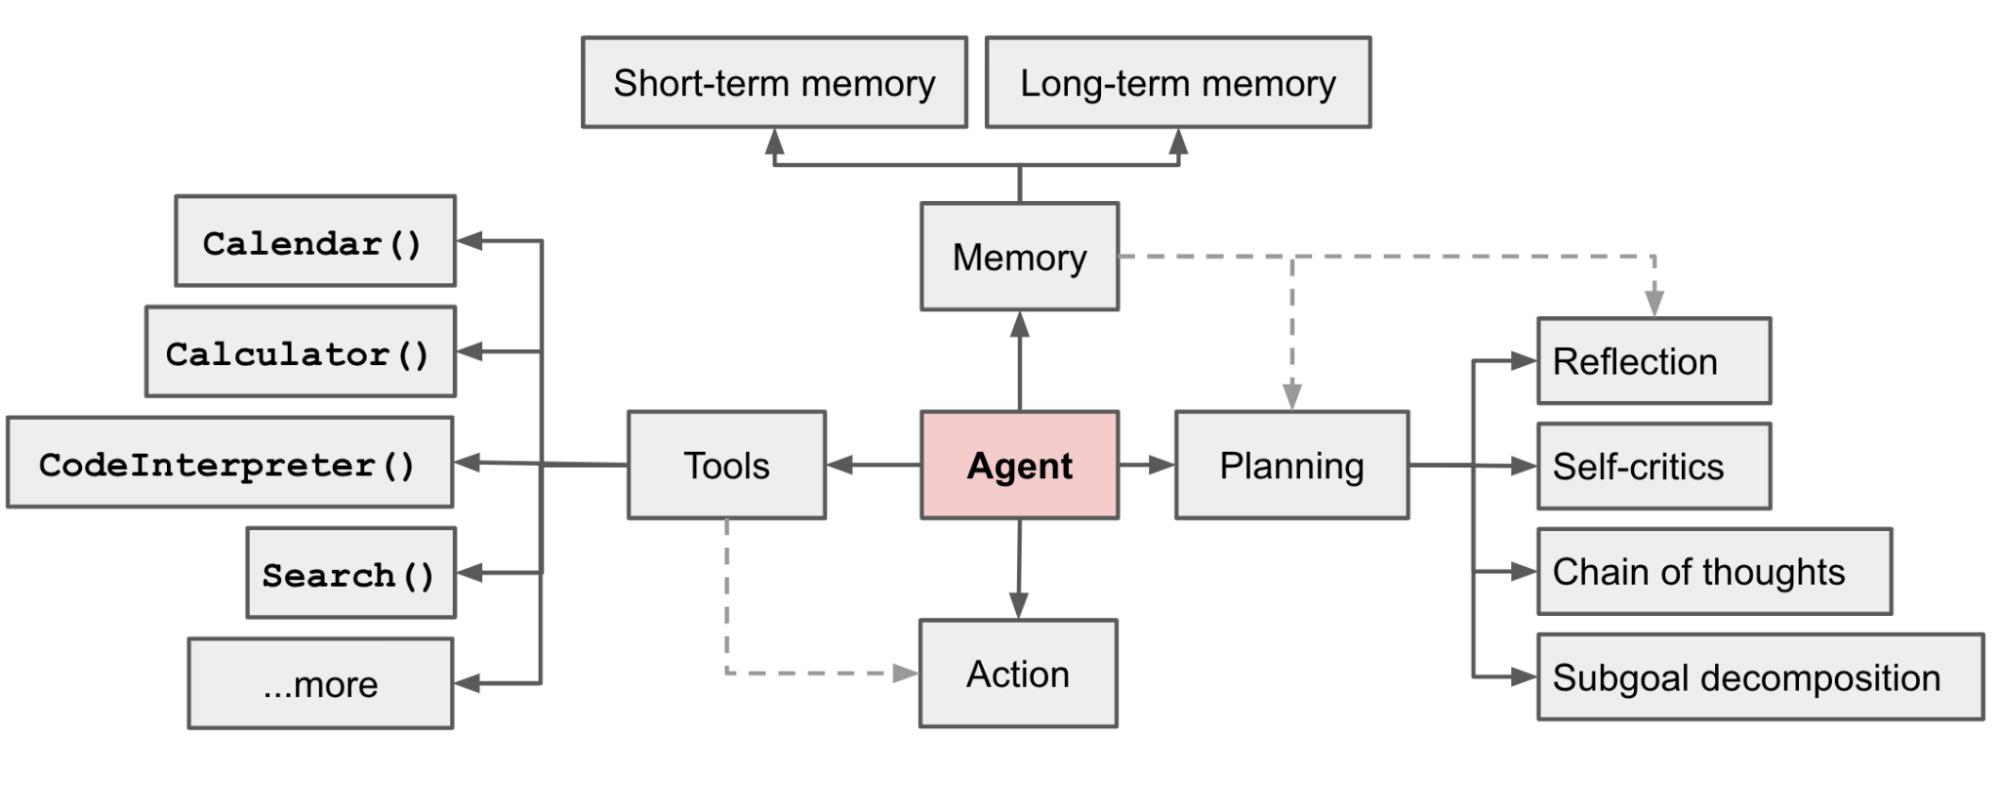
\includegraphics[width=0.85\linewidth]{images/ai/Tools.png} % Replace with your actual image file
  \caption{AI Agent Tool-Calling Architecture.}
  \label{fig:ai-agent-tools}
\end{figure}

Work such as Toolformer demonstrates that models can be trained in a largely self-supervised fashion to identify beneficial tool call sites and to rewrite prompts so that the tool output improves downstream language modeling likelihood; the Toolformer objective augments the base language modeling objective with a selection criterion that promotes tool calls that increase predictive utility \cite{schick23}.  This meta-learning of tool usage is powerful because it combines the flexible, generalizable reasoning of a neural model with the deterministic correctness of specialized utilities.

\paragraph{Safety and validation.} Tool invocation requires defensible safety mechanisms.  Middleware typically implements (i) schema validation on arguments before invocation, (ii) sandboxing and resource limits during execution, and (iii) post-invocation verification (e.g., cross-checking computational results or enforcing type/format invariants) prior to re-inserting outputs into the model context.

\subsection{Multi-agent environments, roles, and emergent coordination}

As a continuation of the architectural patterns surveyed above (single-model policies, planner–executor decompositions, and tool-augmented hybrids), recent work situates those agent designs inside \emph{multi-agent systems} (MAS) constructed from LLMs. In this paradigm, an LLM is no longer only an isolated decision maker but a node in a network of interacting agents that exchange messages, coordinate on subtasks, share memory, and jointly form world models. Research converges on several core design dimensions that determine the behavior, scalability, and interpretability of LLM-based MAS: (1) specification of agent \emph{profiles} (capabilities, tool sets, priors, and prompt templates); (2) selection of \emph{interaction topologies} (who can talk to whom and when); (3) communication protocol design (natural language vs. structured schemas, synchronous vs. asynchronous messaging); (4) environment and world-model fidelity (abstract dialogue arenas vs. embodied or web-like environments); and (5) metrics and theoretical constructs for quantifying emergent collective properties such as synergy, division of labor, and coalition formation \cite{agentic_survey}.

Multi-agent LLM research uses a range of environment models that vary by fidelity, observability, and action expressiveness. At one end are \emph{abstract dialogue arenas}: controlled, language-only settings in which agents exchange messages, negotiate plans, or play coordination games. At the other end are \emph{embodied} or \emph{web-like} environments where agents manipulate objects, navigate interfaces, or perform multi-step tasks requiring grounding, tool invocation, and state tracking. Representative platforms include TextWorld, ALFWorld, and WebArena . Formally, a multi-agent environment can be described as a stochastic game $(\mathcal{S}, \mathcal{A}_1,\dots,\mathcal{A}_n, P, R_1,\dots,R_n)$, where $\mathcal{S}$ is the global state space, $\mathcal{A}_i$ the action space of agent $i$, $P$ the transition kernel $P(s_{t+1}\mid s_t, a_{1,t},\dots,a_{n,t})$, and $R_i$ the reward function for agent $i$ \cite{stochastic_game_LLM}. For LLM agents, the action space $\mathcal{A}_i$ is hybrid: (i) natural-language utterances $u\in\mathcal{U}$, (ii) structured messages (JSON/Protobuf payloads), and (iii) tool invocations $t\in\mathcal{T}$. Observations are typically partial: $o_{i,t} = \mathcal{O}_i(s_t)$, and the LLM-based policy is $\pi_{\theta_i}(a_{i,t}\mid h_{i,t})$, where $h_{i,t}$ merges observations, memory, role prompt, and tool outputs.

Functional specialization is a recurring pattern: agents are assigned roles—planner, critic, executor, retriever, summarizer, tool-wrapper, user proxy—that map to distinct prompts, tool permissions, and priors. Each agent $i$ has a profile $P_i = (\mathcal{C}_i, \mathcal{T}_i, \pi_{\theta_i}^{\mathrm{init}})$. Tasks $T$ can be decomposed into subtasks $T=\bigcup_j t_j$ and allocated via $A: \{t_j\} \to \{1,\dots,n\}$. Explicit role definitions improve throughput and correctness compared to homogeneous teams. Systems like HuggingGPT and AutoGen exemplify planner/selector/executor decompositions, orchestrating specialized agents \cite{hugginggpt, autogen}. The team policy can be expressed as
\[
\Pi((a_{1,t},\dots,a_{n,t})\mid h_{1,t},\dots,h_{n,t}) = \mathcal{C}\big(\pi_{\theta_1}(a_{1,t}\mid h_{1,t}),\dots,\pi_{\theta_n}(a_{n,t}\mid h_{n,t})\big),
\]
where $\mathcal{C}$ enforces coordination constraints.

A principal research question is whether LLM-based MAS produce \emph{emergent} behaviors beyond individual capabilities. Information-theoretic tools such as Partial Information Decomposition (PID) quantify synergy by decomposing predictive information into unique, redundant, and synergistic components across agents’ message streams. Empirical results suggest that shared rewards, repeated interactions, and role heterogeneity promote measurable synergy and emergent communication protocols.

\subsection{Communication in Multi-Agent LLM Systems: Protocols, Emergent Languages, and Grounding}

Communication is the operational substrate of coordination in LLM-based multi-agent systems (LLM-MAS). In these systems, the efficacy of task decomposition, planning, and execution hinges on how agents exchange information, propagate state updates, and negotiate subtasks. From an engineering perspective, communication is both a design choice—human-readable natural language versus structured machine-readable payloads—and a learning phenomenon—agents may develop emergent protocols that optimize efficiency over interpretability. The interplay between these dimensions depends on the use case, safety and interpretability requirements, and environment information structure.

\subsubsection{Communication modalities and message schemas}

Two canonical modalities dominate contemporary LLM-MAS implementations:

\paragraph{Natural-language messaging.} Agents exchange text in human languages (e.g., English). Advantages include interpretability, auditability, and the ability for human overseers to intervene in real time. However, natural language introduces inherent ambiguity, verbosity, and potential misalignment with formalized actions. To mitigate these issues while preserving interpretability, many systems adopt templated messages or structured-natural hybrids. For example, responses may include a machine-parseable JSON snippet preceded or followed by natural-language explanation. Formally, let $m_{i,t} = \text{NL+JSON}(a_{i,t}, r_{i,t})$ be the message generated by agent $i$ at time $t$, where $a_{i,t}$ is the intended action and $r_{i,t}$ is the human-readable rationale. This approach underpins frameworks such as AutoGen and HuggingGPT \cite{autogen, hugginggpt, agentic_survey}.

\paragraph{Structured messaging.} Structured messages encapsulate actions, subtask proposals, beliefs, or state updates in formats such as JSON or Protobuf. Formally, an agent’s message $m_{i,t} \in \mathcal{M}_i$ must satisfy a schema $\mathcal{S}_i$ and can be deterministically parsed into action sequences:
\[
\mathcal{F}_i: m_{i,t} \mapsto \{a_{i,t}^{(1)},\dots,a_{i,t}^{(k)}\}.
\]
Structured messaging reduces ambiguity, supports formal verification, and enables safe execution of tool invocations. Hybrid approaches—structured payloads augmented with natural-language summaries—combine auditability and machine safety, allowing human interpreters to review agent reasoning while automated processes consume formal payloads \cite{schick23}.

\subsubsection{Emergent communication and agent protocol learning}

Emergent communication studies in LLM-MAS extend classical referential games and signaling theory to the context of pre-trained language priors. When agents repeatedly interact under bandwidth constraints, efficiency pressures, or task-specific rewards, they may develop compressed, idiosyncratic protocols $E:\mathcal{H}_{i,t}\mapsto m_{i,t}$ that diverge from human language. Here $\mathcal{H}_{i,t}$ represents the agent’s interaction history, memory, and retrieved context. Iterated learning and generative pressures amplify inductive biases learned during pretraining, producing structured, compositional codes optimized for internal model representations. Empirical studies demonstrate that these protocols often exhibit:
\begin{itemize}
    \item \textbf{Compression and efficiency}: messages minimize token length while maximizing actionable content.
    \item \textbf{Task-specific syntax}: emergent grammars are tailored to internal reasoning chains and tool invocation sequences.
    \item \textbf{Opacity to humans}: while efficient, emergent codes may be unintelligible without translation layers.
\end{itemize}
Design tradeoffs must balance interpretability and efficiency. Constraining agents to human-readable formats preserves auditability, essential in domains such as clinical decision support, finance, or customer automation. Allowing controlled emergent protocols can improve throughput in internal pipelines but requires monitoring, translation agents, or intermittent supervision to ensure traceability \cite{emergent_coordination}.



The formal study of communication in LLM-MAS therefore spans hybrid message design, emergent protocol learning, and strategic interactions. By integrating these perspectives, system designers can craft agents that communicate efficiently, maintain safety, and adapt dynamically to multi-agent coordination challenges.
\subsection{AutoGen framework}
\label{sec:autogen_deepdive}

AutoGen is an open-source, research-grade multi-agent conversation framework developed to enable complex LLM applications where multiple agents converse, invoke tools, and cooperate to achieve high-level goals. The AutoGen technical report and accompanying documentation describe the framework primitives, conversation orchestration, memory and tool integration, and practical implementation patterns; the exposition below synthesizes those descriptions and makes explicit the engineering and algorithmic structure underlying AutoGen's design \cite{autogen_arXiv, autogen_ms, autogen_github}.
\begin{figure}[htbp]
    \centering
    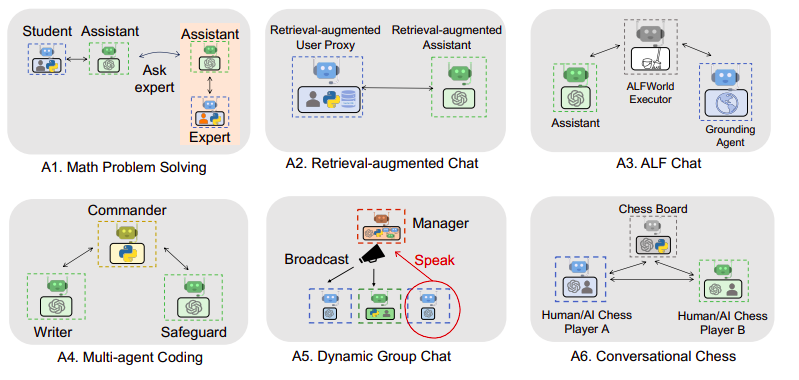
\includegraphics[width=0.8\textwidth]{images/ai/Autogen_agent.png}
    \caption{Examples of AutoGen multi-agent interaction diagram.}
    \label{fig:autogen_architecture}
\end{figure}
\subsubsection{AutoGen core architecture and abstractions}
\label{sec:autogen_core}

AutoGen's runtime is organized around a small set of first-class abstractions that map directly to conversation programming constructs and to the LLM prompting pipeline:

\begin{itemize}
  \item \textbf{Agent.} An \emph{agent} is a composable object encapsulating (i) a \emph{role profile} (system prompt template, instruction scaffolding, and model configuration); (ii) a \emph{tool registry} (a set of authorized external functions/APIs with type signatures); and (iii) a \emph{memory interface} (episodic logs, summaries, or handles to persistent vector stores). Agents are interoperable: a single LLM backbone can instantiate multiple agents by switching role templates and tool permissions at runtime. Agents may be executed locally or via external LLM APIs. The AutoGen paper formalizes agents as tuples \(A_i=(R_i,\mathcal{T}_i,\mathcal{M}_i,\lambda_i)\) where \(R_i\) is the role prompt, \(\mathcal{T}_i\) the tool set, \(\mathcal{M}_i\) the memory access interface, and \(\lambda_i\) the model invocation parameters (temperature, max tokens, stop tokens). \cite{autogen_arXiv}
  \item \textbf{Dialogue/Conversation Manager.} The Conversation Manager (CM) is the orchestration layer that (a) schedules turns among agents, (b) constructs per-turn prompts by merging role prompts, recent dialogue, and retrieved memory, (c) validates and parses agent outputs, and (d) mediates tool invocation and result reinsertion. The CM implements pluggable scheduling policies (round-robin, priority queues, event triggers) and ensures token-budget and API-call budgets are respected. \cite{autogen_arXiv, autogen_github}
  \item \textbf{Tool / Plugin Interface.} Tools are registered with signatures and safety metadata. The CM maps structured tokens emitted by agents (e.g., well-formed JSON) to tool calls and routes responses back into the conversation context. Tool execution occurs in sandboxed runtimes with pre/post-condition checks and resource limits (timeouts, memory caps). \cite{autogen_arXiv}
  \item \textbf{Memory Stores.} AutoGen supports pluggable backends (in-memory logs, persistent text stores, and vector indices). Memory is structured into layers—episodic history, compressed summaries, and semantic indices for retrieval. The CM exposes retrieval APIs used in prompt construction and implements background compaction/summarization pipelines to keep the prompt footprint manageable. \cite{autogen_arXiv, autogen_github}
  \item \textbf{Message Schemas and Validators.} AutoGen encourages schema-driven exchanges. Agents are expected to emit outputs conforming to developer-declared JSON/Protobuf schemas; the CM validates outputs and applies fallback corrective strategies if validation fails (clarification request, heuristic repair, verifier invocation). \cite{autogen_arXiv}
\end{itemize}

These abstractions convert conversational programming tasks into a disciplined prompt-construction and execution pipeline: when it is an agent's turn, the CM computes a prompt \(P\) by composing the agent's role prompt \(R_i\), the retrieved memory \(M_{\mathrm{ret}}\), and recent dialogue \(H_{\mathrm{recent}}\); then the LLM is invoked to produce a token sequence that is post-processed into actions or tool calls.



\subsubsection{Conversation orchestration logic}
\label{sec:autogen_orchestration}

AutoGen conceptualizes multi-agent coordination in terms of a small set of reusable \emph{conversation patterns}. Each pattern specifies how turns are selected, how context is propagated across interactions, and how intermediate state is summarized and reused. Rather than exposing a single low-level scheduling loop, AutoGen emphasizes higher-level abstractions that balance modularity, controllability, and cost efficiency.

The AutoGen framework identifies several canonical interaction patterns:

\begin{itemize}
  \item \textbf{Two-agent conversation.} The simplest pattern involves a pair of agents engaging in a bounded multi-turn dialogue, typically initiated via an explicit chat invocation. The result of such a conversation is encapsulated in a structured artifact that includes the full message trace, a concise summary, and token or cost statistics. This pattern is well suited for focused subproblems or bilateral reasoning.
\begin{figure}[t]
  \centering
  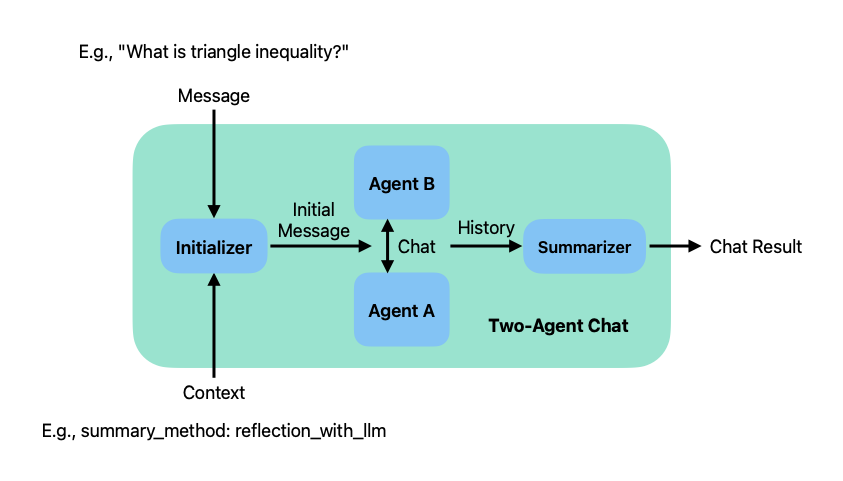
\includegraphics[width=0.85\linewidth]{images/ai/Two_Agents_chat.png}
  \caption{Two-agent conversation pattern}
  \label{fig:two_agents_conversation}
\end{figure}

  \item \textbf{Sequential (carryover) conversations.} More complex workflows are expressed as a sequence of two-agent conversations, where each interaction produces a summary that is injected as carryover context into the subsequent one. This enables staged task decomposition (e.g., analysis $\rightarrow$ planning $\rightarrow$ execution) while controlling context growth through configurable summarization policies.
\begin{figure}[t]
  \centering
  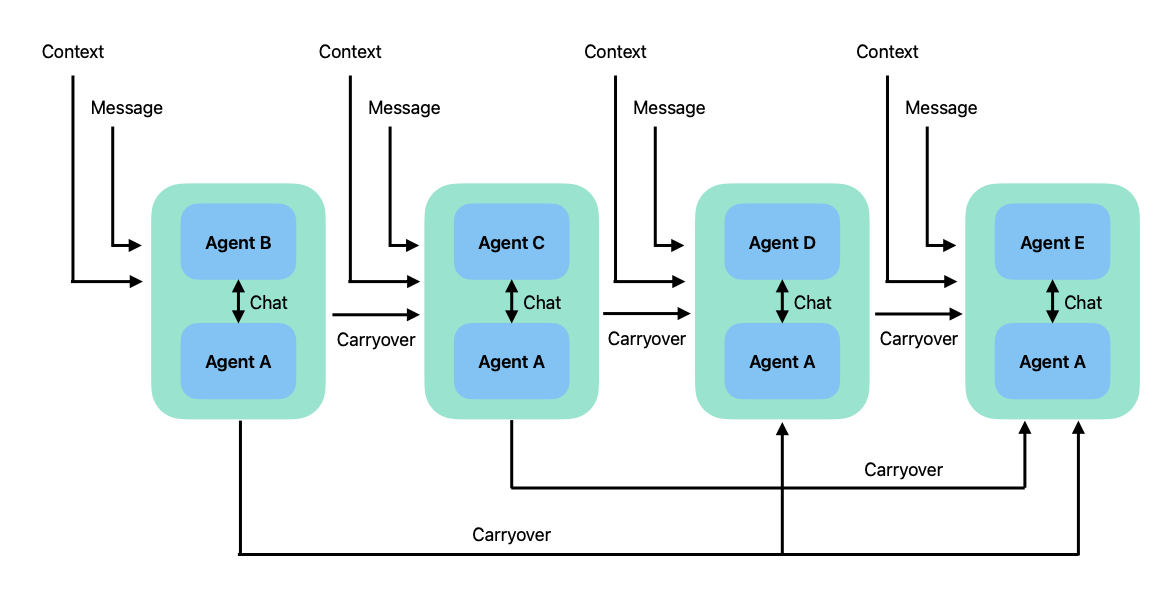
\includegraphics[width=0.85\linewidth]{images/ai/Sequential_chat.png}
  \caption{Sequential converstation pattern}
  \label{fig:sequential_conversation}
\end{figure}

  \item \textbf{Group conversations.} In this pattern, multiple agents participate in a shared dialogue. A central design choice concerns \paragraph{speaker selection}: In group conversations, AutoGen delegates turn-taking to a \emph{Group Chat Manager}, which is responsible for selecting the next speaking agent according to a configurable strategy. Currently supported strategies include: \emph{round\_robin}, which deterministically cycles through agents in a fixed order; \emph{random}, which samples the next agent uniformly at random; \emph{manual}, in which turn selection is deferred to human input; and \emph{auto}, the default strategy, where an LLM-based policy selects the next agent based on the evolving conversational context. These strategies offer a spectrum of trade-offs between determinism, human oversight, flexibility, and computational cost, and may be combined with additional constraints or custom selection functions to enforce domain-specific interaction policies..
\begin{figure}[t]
  \centering
  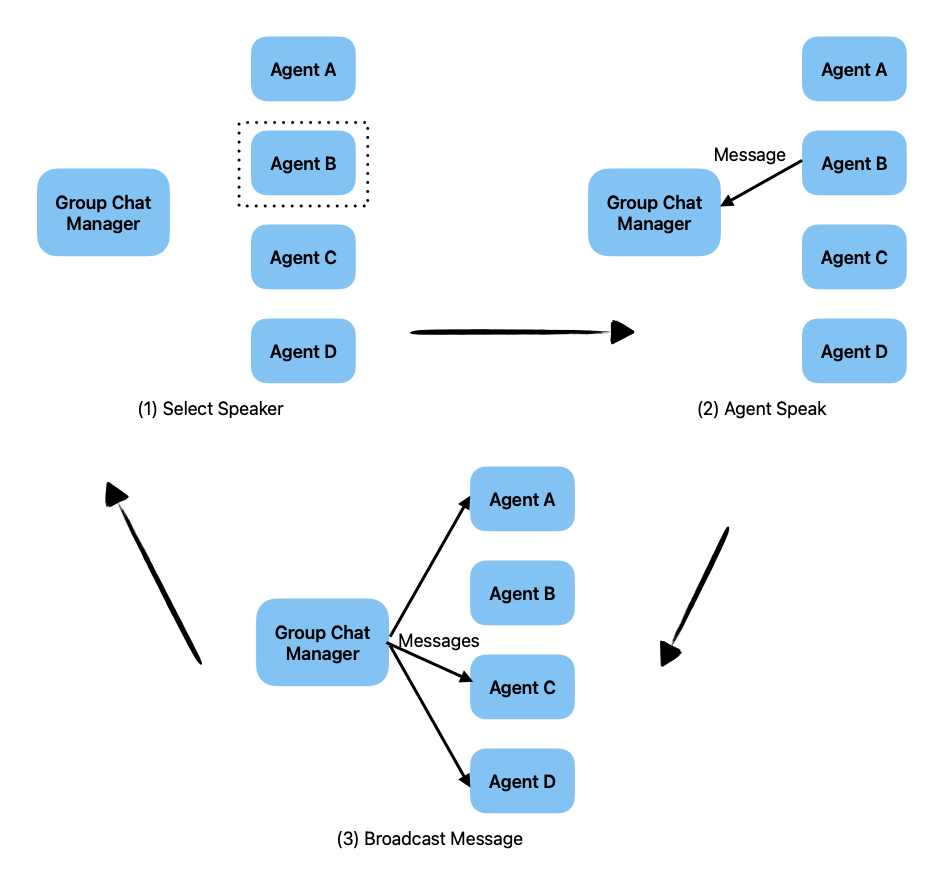
\includegraphics[width=0.85\linewidth]{images/ai/Group_Chat.png}
  \caption{Group conversation pattern}
  \label{fig:group_chat_conversation}
\end{figure}

  \item \textbf{Nested conversations.} Nested or packaged conversations encapsulate an internal multi-agent workflow behind a single agent interface. From the perspective of the outer orchestration layer, the nested workflow behaves as a single agent, enabling hierarchical composition and reuse of common interaction templates.

\end{itemize}


\paragraph{Design considerations.}
The choice of conversation pattern depends on the structure of the task and operational constraints. Two-agent and unconstrained group conversations favor flexibility and exploratory reasoning, whereas sequential and constrained group patterns support predictable pipelines and bounded costs. Nested conversations facilitate modular system design by isolating complexity and promoting reuse.

Overall, AutoGen’s conversation patterns provide a declarative layer for multi-agent orchestration, shifting the focus from low-level scheduling mechanics to higher-level interaction design and enabling systematic reasoning about cost, context, and control.

\subsubsection{Tool integration and verification}
\label{sec:autogen_tools}

AutoGen treats tools as typed, sandboxed functions. Tool registration includes a name, a typed signature, resource constraints, and an optional validator. The mapping from textual output to a tool invocation is mediated by a parser \( \mathcal{P}\) that extracts structured arguments from the produced tokens. The tool invocation pipeline is:

\[
\text{tokens} \xrightarrow{\ \mathcal{P}\ } \text{args} \xrightarrow{\ \text{schema\_check}\ } \text{call}\xrightarrow{\ \text{sandbox}\ } \text{result} \xrightarrow{\ \text{postprocess}\ } \text{context\_update}.
\]

Key safety primitives described in the AutoGen report are:

\begin{itemize}
  \item \textbf{Pre-condition / schema checks:} require tool arguments to satisfy developer-declared invariants prior to execution.
  \item \textbf{Sandboxing:} run untrusted code and resource-heavy tools within containerized, time-boxed environments to limit side-effects.
  \item \textbf{Post-condition validation:} verify result types and ranges before merging outputs into agent contexts; if validation fails, flag to verifier agents or request agent clarification.
\end{itemize}

AutoGen documents practical examples where tool outputs are immediately embedded into the conversation and re-tokenized for subsequent reasoning (e.g., code execution results, database query responses). The framework supports serializing tool outputs both as human-readable summaries and as vector embeddings for retrieval.

\subsubsection{Memory architecture and retrieval}
\label{sec:autogen_memory}

AutoGen adopts a multi-tier memory model:

\begin{description}
  \item[Episodic memory:] the raw conversation log (recent $n$ turns). Used for short-term coherence and context.
  \item[Semantic summaries:] periodic LLM-produced summaries that compress long histories into concise artifacts for long-horizon tasks.
  \item[Indexed semantic store:] vector embeddings of important artifacts (summaries, tool outputs, factual assertions) stored in an ANN index (approximate nearest neighbor) for retrieval-augmented prompting.
\end{description}

Retrieval forms an explicit stage in prompt construction. Given a retrieval query derived from current goal \(g\), the CM performs:

\[
M_{\mathrm{ret}} = \text{TopK}_{\mathrm{ANN}}\big(\mathrm{embed}(q(g)),\; k\big)
\]

and inserts the canonicalized textual summaries of \(M_{\mathrm{ret}}\) into the agent prompt. The report emphasizes cost-aware retrieval: selecting top-k that maximize relevance while satisfying token budget constraints (e.g., prefer compressed summaries over raw long dialogues). AutoGen also supports retention policies and scheduled summarization routines to limit unbounded growth of stored artifacts. \cite{autogen_arXiv, autogen_github}

 AutoGen formalizes a conversation-first programming model that maps naturally to contemporary LLM capabilities: it treats agents as role-templated LLM instances with controlled tool access, it enforces schema validation and sandboxed tool execution for safety, and it places memory retrieval and cost-aware prompt assembly at the heart of the orchestration pipeline. The framework's modular abstractions and rich developer tooling have enabled reproducible research on agentic workflows while illuminating practical tradeoffs (cost, latency, hallucination) that remain active areas of investigation.

\section{Retrieval‑Augmented Generation}

Retrieval-Augmented Generation (RAG) is a hybrid framework in natural language processing that integrates external information retrieval with large pretrained generative models, enabling the model to dynamically fetch relevant documents from a knowledge corpus and condition its responses on that retrieved content \cite{lewis20}. This approach was introduced to address limitations of conventional generative language models, such as static knowledge confined to training data, difficulty in updating world information, lack of provenance for generated facts, and poor performance on knowledge-intensive tasks \cite{lewis20}. By combining parametric memory (the generative model) with non-parametric memory (an external retriever and index), RAG improves factual accuracy, reduces hallucinations, and allows the model to provide more contextually informed outputs, making it particularly effective for tasks such as open-domain question answering, summarization, and knowledge-grounded dialogue \cite{schick23, yao22}.

\begin{figure}[t]
  \centering
  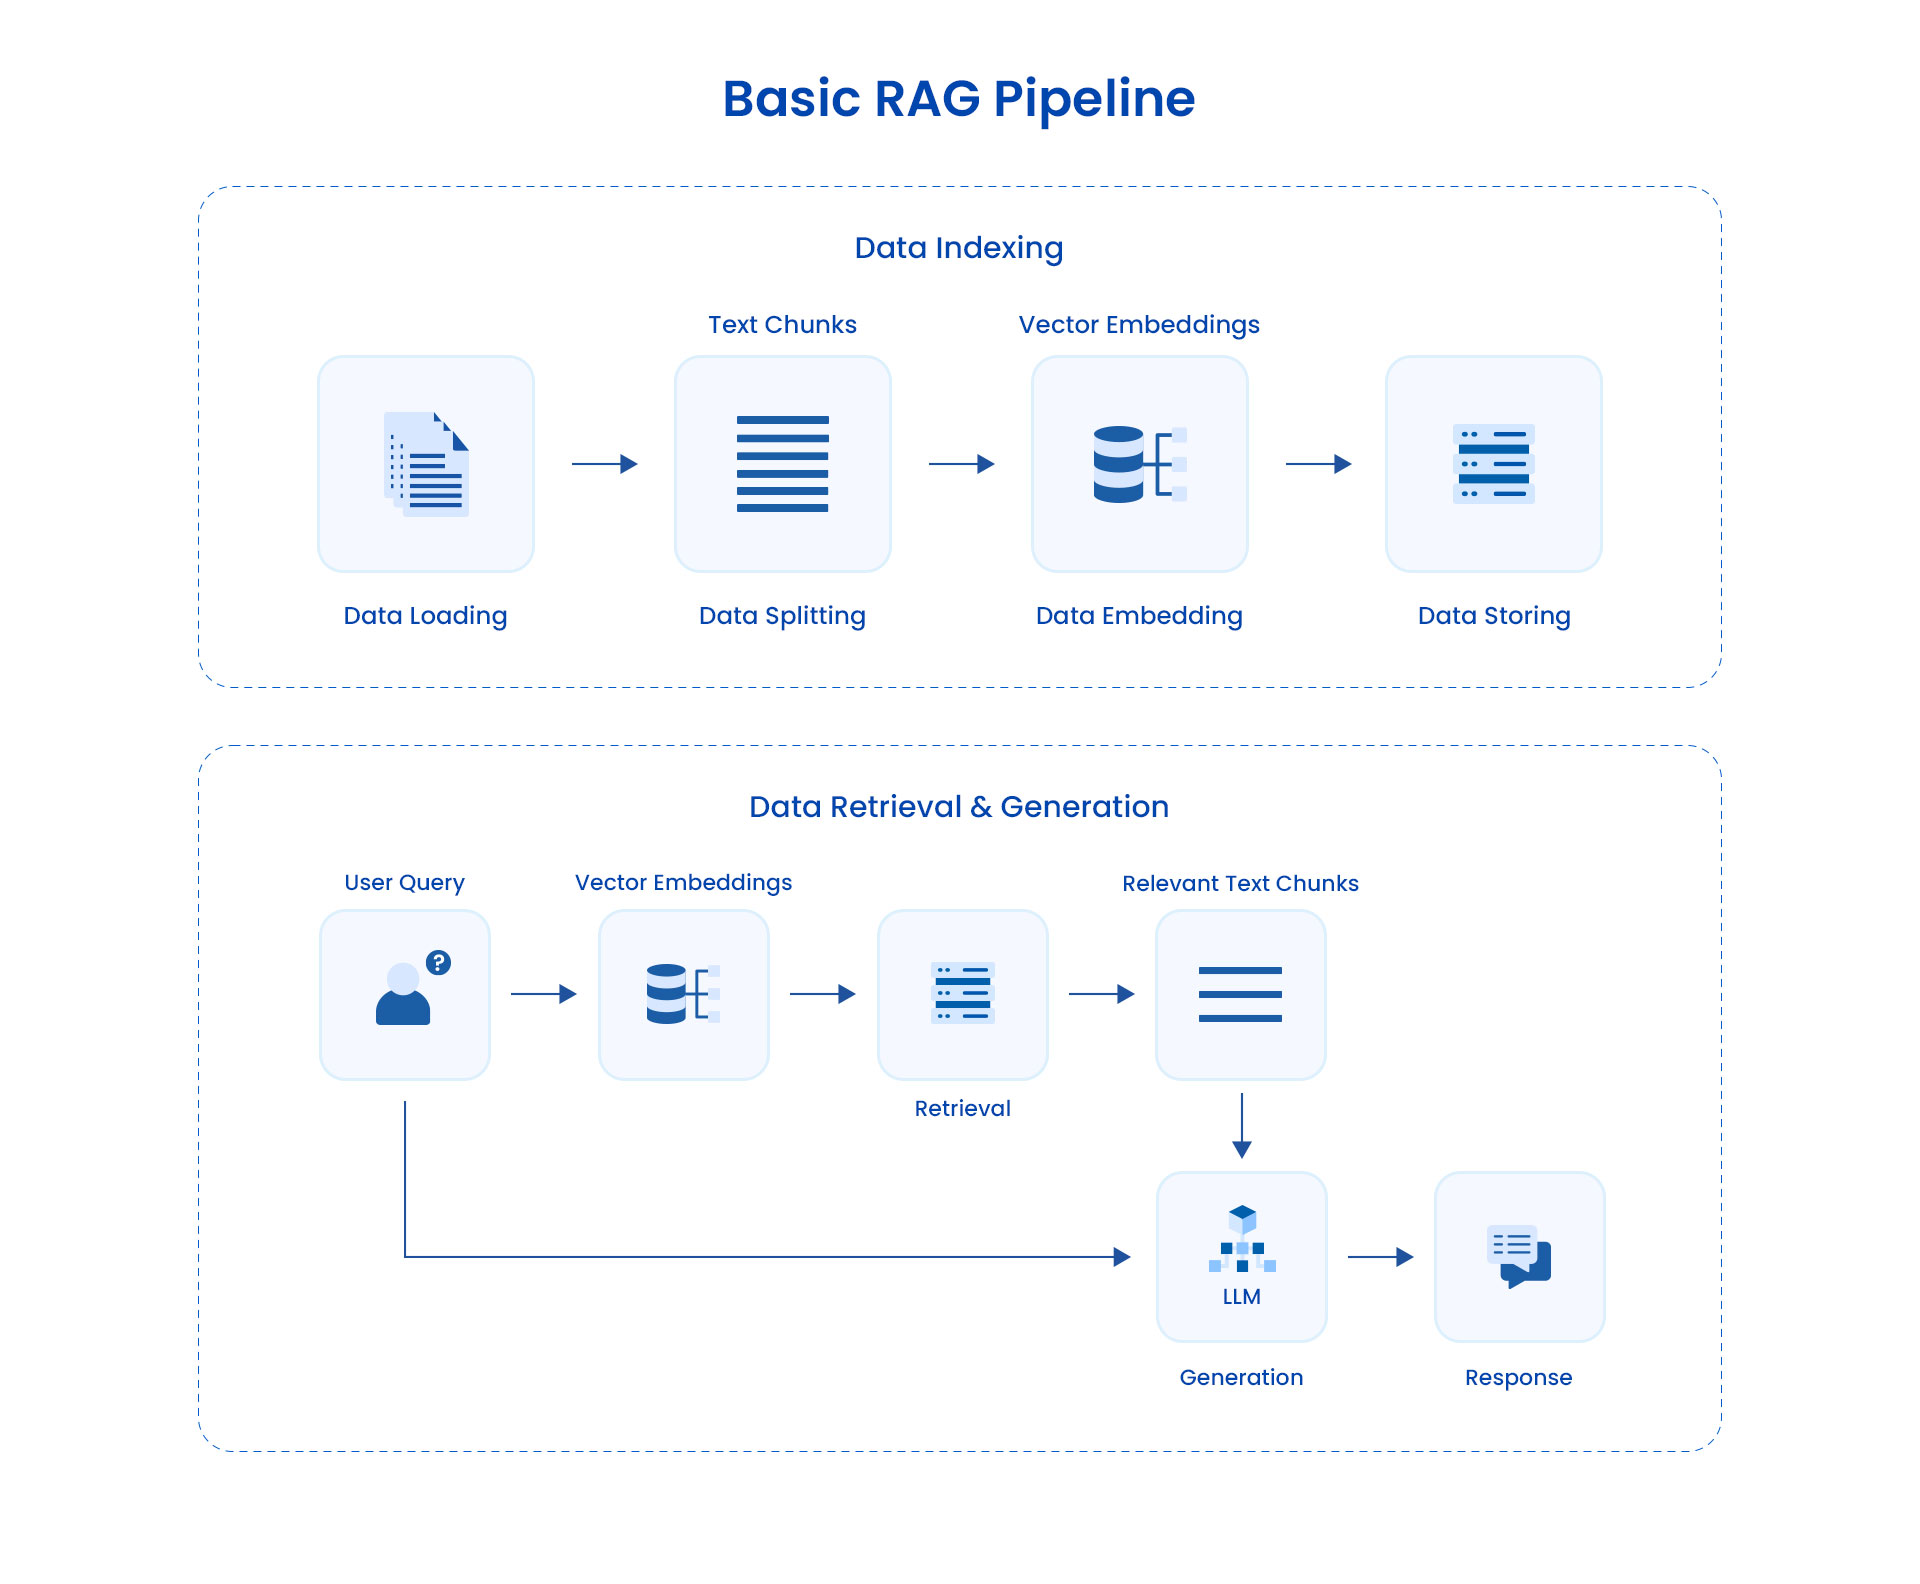
\includegraphics[width=0.85\linewidth]{images/ai/RAG.jpg}
  \caption{Simple Retrieval-Augmented Generation Pipeline}
  \label{fig:rag_pipeline}
\end{figure}




